\NeedsTeXFormat{LaTeX2e}[2005/12/01]
%%    2010/04/06 v1.0 Vorlage Master-Forschungspraktikum Versuchsauswertung
%%    based on the 2009/10/14 v0.1 GAUBM template by Prof Pruschke

\documentclass[twoside,        %% zweiseitiges Layout
               BCOR12mm,       %% Bindekorrektur 12 mm
% please comment out if report is in English
               english,ngerman, %% Dokumentspr. Deutsch, Alternativspr. Englisch
% please remove comment if report is in English 
%               ngerman,english, %% Dokumentspr. Englisch, Alternativspr. Deutsch
               fleqn,headsepline=false,footsepline=false
              ]{MFPREPORT}

%% Pakete und Definitionen ausgelagert
\usepackage{a4}
\usepackage{multicol}

% language option set in JGNSUM class
\usepackage{babel}
\usepackage{hyperref}

%% FONT:
%\usepackage{lmodern}
\usepackage{times} % sieht besser aus als lmodern
%\usepackage{palatino} % sieht schlechter aus als times
%\usepackage{mathpazo} % very ugly font, to be loaded later ???
%\usepackage{cmbright} % doesn't work either
\usepackage[T1]{fontenc}
\usepackage{textcomp}

\usepackage{ucs}
\usepackage[utf8x]{inputenc}

\usepackage{amsfonts}
\usepackage{amstext}
\usepackage{amsmath}
\usepackage{amsthm}
\usepackage{amssymb}
\usepackage{amsbsy}   % AMS-Boldsymbol

% \usepackage{mathabx} % e.g. for \Sun
%% but not a standard package (neither texlive nor Miktex)
%% so use wasysym (\astrosun) instead
\usepackage{wasysym} % e.g. for \astrosun or \CheckedBox

\usepackage{bbm,mathrsfs}

\usepackage{textcomp} % noch einige coole symbole

\usepackage{sectsty}
\allsectionsfont{\raggedright}

\usepackage[numbers]{natbib}
\citestyle{dinat}
\bibliographystyle{dinat}

\usepackage{makeidx}

\usepackage{url}	% für hübsche URLs mit Link
\usepackage{color}	% für farben a la \definecolor{Gray}{gray}{0.5}
\usepackage{verbatim}
\usepackage{subfigure}
\usepackage{listings}

\usepackage{fancybox}
%usage:
%\begin{Verbatim}[frame=single,label=Titel]
%Verbatim Zeile
%\end{Verbatim}


 \setlength{\textwidth}{16.2cm}
 \setlength{\textheight}{24cm}
 \setlength{\oddsidemargin}{0cm}
 \setlength{\evensidemargin}{-0.5cm}

 %unbedingt nach abmessungen einfügen!
 \usepackage{fancyhdr}
 \pagestyle{fancy}
 %\sloppy % für weniger absatzfehler

 \setcounter{tocdepth}{2}
 \setcounter{secnumdepth}{2}

 \ifreportelse{\numberwithin{equation}{chapter}}{\numberwithin{equation}{section}}
 \theoremstyle{plain}% default
 \ifreportelse{\newtheorem{thm}{Theorem}[chapter]}{\newtheorem{thm}{Theorem}[section]}

 \newtheorem{satz}{Satz}
 \newtheorem{lem}[thm]{Lemma}
 \newtheorem{prop}[thm]{Proposition}
 \newtheorem{kor}[thm]{Korollar}
 \newtheorem{cor}[thm]{Corollary}

 \theoremstyle{definition}
 \newtheorem{defi}{Definition}

 \def\@proof{%
  \if@englishpreamble{Proof}\else{Beweis}\fi
 }
 \newenvironment{bew}{\begin{proof}[\@proof]}{\end{proof}}



%% einbinden einiger nützlicher Befehle
\newcommand{\iflanggerman}[2]{
 \iflanguage{german}{#1}{
  \iflanguage{ngerman}{#1}{#2}
 }
}

% box around the whole equation, number inclusive
\newcommand{\boxedeqn}[1]{%
  \[\fbox{%
      \addtolength{\linewidth}{-2\fboxsep}%
      \addtolength{\linewidth}{-2\fboxrule}%
      \begin{minipage}{\linewidth}%
      \begin{equation}#1\end{equation}%
      \end{minipage}%
    }\]%
}

\iflanggerman{
 \newcommand{\const}{\mathrm{konst}}
 \newcommand{\Const}{\mathrm{konst.}}
}{
 \newcommand{\const}{\mathrm{const}}
 \newcommand{\Const}{\mathrm{const.}}
}

% von Meier
\newcommand{\nbd}{\nobreakdash-\hspace{0pt}}
% example: $K$\nbd{}Vektorraum
\newcommand*{\transpose}[1]{\prescript{t}{}{#1}}
\newcommand*{\conjugate}[1]{\overline{#1}}
\newcommand*{\abs}[1]{\lvert#1\rvert}
\newcommand*{\Mod}{\mathrm{mod}}
\newcommand{\symdif}{\mathbin\triangle}
\DeclareMathOperator{\Graph}{Graph}
\DeclareMathOperator{\id}{id}
\DeclareMathOperator*{\grad}{grad}
\DeclareMathOperator*{\Div}{div}
\DeclareMathOperator*{\rot}{rot}
\DeclareMathOperator{\sig}{sig}
\DeclareMathOperator{\sgn}{sgn}
\DeclareMathOperator{\diag}{diag}
\DeclareMathOperator{\tr}{tr}
\DeclareMathOperator{\Sp}{Sp}
\DeclareMathOperator{\im}{Im}
\DeclareMathOperator{\re}{Re}

\newcommand{\vcentcolon}{\mathop{:}}



\begin{document}
\LabratoryName{AG.TIM}{Numerische Simulationen von Turbulenz im interstellaren Medium}
\ProtocolAuthor{Mein Vorname}{Nachname}{meine@email}
\Assistant{Betr. Vorname}{Nachname}
\ResearchFocus{Astro- und Geophysik (M.phy.401)}
% In der naechsten Version beruecksichtigt
%\Collaborator{Vorname}{Nachname}{email}
\ConductedOn{15}{4}{2010}
\date{\today}
% eines von beiden
\CopyNotWanted
%\CopyWanted

\pagenumbering{roman}
\maketitle

%\begin{otherlanguage}{english}
%\end{otherlanguage}

\tableofcontents

\clearpage
\pagenumbering{arabic}

\section{Einleitung}
Hier geht es los. Bitte alle Quellen (auch Internetseiten) angeben.


\section{Theorie}

\subsection{Grundbegriffe}
An dieser Stelle ist es sinnvoll kurz auf
einige immer wieder auftauchende Grundbegriffe der hier untersuchten Physik einzugehen.








\paragraph{Die Zustandsdichte $D(E)$} gibt an wieviele Zustande in einem gegebenem Energie $dE$ oder auch Impulsintervall $d p$ liegen.
Abhängig von der Dimension besitzt die Zustandsdichte die Elektronen (Fermionen) eine andere Form. 
In den für uns wichtigen drei Dimensionen ergibt sich:
\begin{align}
D(E) = \sum_{\sigma} \frac{(2m^{*})^{\frac{3}{2}}}{2 \pi^2 \hbar^3} \sqrt{E}
\end{align}
Es muss zudem, wie angedeutet über Spin $\sigma=\lbrace \uparrow, \downarrow \rbrace$ summiert werden.
Wie üblich zieht man zur Beschriebung der Elektronen das Modell der effektiven Masse $m^{*}$ heran und setzt dabei vorraus dass sie eine parabolische Dispersionsrelation erfüllen.
\\
\paragraph{Die Fermiverteilung $f_{T,\mu}(E)$} gibt im Falle der Näherung freier nicht wechselwirkender und ausschließlich dem Pauli-Prinzip genügender Spin $\sigma = \frac{1}{2}$ Teilchen die Wahrscheinlichkeit an, dass ein Zustand der Energie $E$ bei einer fixen bestimmten Temperatur $T$ sowie chemischen Potenzial $\mu$ besetzt ist. 
Das Pauli prinzip besagt, dass nicht zwei Elektronen in allen Quantenzahlen übereinstimmen dürfen. Ausgehend von dieser Zwangsbedingung findet man durch eine statistische Betrachtung die Verteilungsfunktion:
\begin{align}
f_{T, \mu} (E)={\frac {1}{e^{(E-\mu )/kT}+1}}
\end{align}
Bei $T=0$ ist $f_{T,\mu}(E)=1$ für $E \leq E_{F} \equiv \text{ Fermiengerie}$, also alle Zustände besetzt und $f_{T,\mu}(E)=0$ für $E > E_{F} $ kein Zustand besetzt. 
Abhängig von $T$ beobachtet man eine schwache Aufweichung der Fermikante. 
Als \paragraph{Besetzungsdichte $\rho$} bezeichnet man, nun da wir die Zustandsdichte $D(E)$ und die Fermiverteilung definiert haben, deren Produkt dessen Integral die tatsächliche Anzahl an Zustanden $N$ angibt:
\begin{align}
N = \int dN = \int_{0}^{\infty} D(E) f_{T,\mu} (E) dE
\end{align}
 
\subsection{Tunneleffekt}
Ein quantenmechanisches Teilchen ($\equiv$ Welle) ist durch seine Wellenlänge und Energie gekennzeichnet. 
Ein freies Elektron, mit kinetischer Energie $T$ dessen Wellenfunktion ebene Wellen sind kann natürlich ein konstantes Potenzial $V_{B}$ mit Länge $d$ überwinden falls $T \geq V_{B}$.
Aus Stetigkeitsbedingungen und der Schrödingergleichung erhält man jedoch auch für $T \leq V_{B}$ eine Transmissionswahrscheinlichkeit ungleich Null
\footnote{Voraussetzung ist weiterhin nach Pauli, dass unbesetzte Zustände voranden sind, in die getunnelt werden kann.} .
Die Amplitude, dessen Quadrat nach Born die Aufenthaltswahrscheinlichkeit angibt fällt dann innerhalb der Barriere exponentiell ab und schließt sich stetig an die auf der anderen Seite austretende ebene Welle an.
\\
Nach der Transmission ist zudem die Wellenlänge $\lambda^{\prime}$ die gleiche wie beim Eintritt $\lambda$.
\\
Dass die Wellenänge der austretenden Welle nicht von der Dicke $d$ abhängt drückt die Energieerhaltung aus,
da für ein freies Teilchen
\begin{align}
E = \frac{h^2}{2 m \lambda^2} = E^{\prime}
\end{align}
gilt.
\\
Jedoch wird die Tunnelwahrscheinlichkeit umso kleiner je größer die Dicke der Tunnelschicht ist.
\\
Diese ist in dem Versuch durch die Dicke $d$ der Aluminiumoxidschicht gegeben die zudem eine später gegebene Breite besitzt.
Dieses ist ein sehr guter Isolator, da es keine freien Zustande im Leitungsband gibt.


\subsection{Cooper Paare}
Das radikal verschiedene Verhalten eines Supraleiters im Vergleich zu einem Ohm'schen Leiter bedeutet, dass hier ein anderer Wechselwirkungsmechanismus vorliegt im Vergleich zu klassischen Leitern.
\\
Im folgenden wird eine mögliche qualitative Erklärung
\footnote{siehe Buckler}
gegeben. 
Für dieses Model betrachten wir ein positiv geladenes Kristall Gitter, wobei wir als grobe Vereinfachung alle Effekte der Valenzelektronen vernachlässigen.
Wir fassen außerdem die Kristallatome als bewegliche positive Ladungswolken auf.
\\
Tritt nun ein Elektron in den Kristall ein so erzeugt dieses eine Verzerrung des Kristalls.
Dies hat zur Folge, dass sich, mit einiger zeitlicher Verzögerung aufgrund der Trägheit (Masse) der Kerne, in der Nähe des Elektrons eine höhere Konzentrations an positiven Landungen befindet. 
\\
Falls nun ein zweites Elektron der Spur des ersten folgt so spürt es die nun induzierte positive Ladung als eine attraktive Wechselwirkung, da das erste Elektron auch ein Stück weit entfent und damit die Coulomb WW klein ist. Zudem tragen die positiven Ladungen zusätzlich mit einer Abschirmung zur Abschwächung der Elektronenabstoßung bei.
Bei einem Supraleiter sind die dadurch entstehenden Anziehungskräfte groß, dass die Abstoßung vergleichsweise klein ist.
\\
Nun wird also eine Art Gleichgewichtszustund erreicht wenn der Abstand der Elektronen gerade der Kohärenzlänge entspricht. 
Diese interpretiert man dann als die Ausdehnung eines neuen Teilchenzustandes, dem Cooper Paar.
\\
Durch theoretische Betrachtungen konnte Cooper zeigen, dass die Gesamtenergie des erwähntes Zweiteilchenzustandes besonders stabil ist, wenn $p_1 = -p_2$. 
\\
Daher wird dieser Zustand bevorzugt angenommen.
Die früher erwähnte Wechselwirkung der Elektronen, die diesen Zustand stabilisiert, wird über Phononen vermittelt.
Diese sind ebenso wie der neue Zustand Quasiteilchen, weil dieser Zustand nur als ein kollektives Phänomen innerhalb des Kristalls auftritt.
Außerdem muss der Spin der Elektronen einander entgegengesetzt sein, weshalb das Cooperpaar einen Gesamtspin Null hat.
\\
Daher genügen die Cooper Paare nicht der Fermi Statistik, was ermöglicht dass alle Paare einen gesamten makroskopischen Zustand bilden können.
\\
Energetisch gesehen liegt dieser kollektive Zustand in der Nähe der Fermi Energie der ungepaarten Elektronen,
da die anderen Zustände bereits besetzt sind.
\\
Hieraus resultiert ein für die ungepaaren Elektronen verbotener Bereich ('Gap') mit der Breite $2 \Delta$, wobei $\Delta$ die Absenkung der Energie bezeichnet, die durch den Cooperzustand erzielt wird.
Um einen gebundenen Zustand aufzubrechen ist nun gerade eine Energie von $2 \Delta$ notwendig.


Desweiteren wird die Zustandsdichte durch die Wechselwirkung der Phononen so verzerrt dass es Zustande geringer Energie von den Elektronen angenommen werden, die vormals im Gap lagen. 
Dies führt zu einer Abnahme der Zustandsdichte in der Nähe der Kante und damit zu charakteristischen Maxima sowie unbesetzen Zuständen.
Der erläuterte Verlauf der Zustandsdichte im Supraleiternden Zustand ist in Grafik... gezeigt.

\subsection{Tunnelkennlinien}

Im folgenden soll es darum gehen die Bandlücke $\Delta$ und damit indirekt den supraleitenden Zustand zu vermessen, um diesen später mit theoretischen Werten zu vergleichen.
\\
Naheliegend wäre es an dieser Stelle ein optisches Experiment durchzuführen, jedoch ist es in der Praxis leichter einen Tunnelstrom zu vermessen.
Der Aufbau ist dabei immer so, dass zwei Schichten (supra-) leiternden Materials durch eine sehr gut isolierende Oxidschicht ($\equiv $ Tunnelbarriere) getrennt sind. 
Nun kann man durch das Anlegen einer Spannung an die beiden leitenden Schichten einen kleinen Tunnelstrom messen der eine Funktion der angelegten Spannung ist ($\equiv$ kinetische Energie der Tunnelelektronen) sowie der Hohe des Potenzialwalls ($\leftrightsquigarrow$ Dicke $d$ der Oxidschicht) welche im wesentlichen die Tunnelwahrscheinlichkeit bestimmt.
\\
Weil es ein einfaches Referenzsystem ist wird zunächst die Tunnelkennlinie für den NL/NL Kontakt diskutiert, siehe dazu Abb. \ref{fig:tunnel1} a.
bevor eine Spannung $U$ angelegt wird befindet sich das System im Gleichgewicht, weshalb gleichviele Elektronen in beide Richtungen tunneln.
Mit angelegter Spannung werden die Fermienergien $E_F$ relativ zu einander verschoben um $e \cdot U$, sodass ein Nettostrom von links nach rechts in freie sowie energietisch niedrig liegendere Zustäde stattfinden kann. 
Da die Verschiebung der Fermikanten und damit die Zahl der potenziell tunnelbaren Zustände direkt propotional ist zur angelegten Spannung $U$ können wir ein ohmsches Verhalten $U= R \cdot I$ für die Kennlinie erwarten (Fig. \ref{fig:tunnel2} a).
Die Temperaturabhängigkeit ist im Regim hoher Temperaturen, weil es dann viele Phononen gibt derart, dass die Leitfähigkeit $\sigma \propto T^{-\frac{3}{2}}$.
\\
Anders verhält es sich bei einem Sandwich aus einem Supraleiter und einem Normalleiter, siehe dazu Fig. \ref{fig:tunnel2} b.
Auffällig ist hier, dass erst an einer charakteristischen Tunnelspannung die genau der Energie des Cooperpaares entpricht, einsetzt. Dies ermöglicht später eine Einschätzung für die Größe der Bandlücke  über $\Delta= e \cdot U_c$. 
\\
Für hohe Stromdichten erkennt man dass der Verlauf sich wieder dem Ohmschen annähert, da für große Elektronengeschwindigkeiten  die Zahl der Cooperpaare abnimmt. Zudem ist die Form der SL/NL Kennlinie auch Temperatur abhängig, denn für $T  \neq 0$ liegt eine leichte Verschmierung der Fermikante im Normalleiter vor und zudem liegen auch manche Elektronen im Supraleiter schon oberhalb der Bandlücke, welche sich zudem verkleinert.
\\
Diese Effekte liegen in der idealisierten dritten Kurve (c) für den absoluten Temperatur Nullpunkt nicht mehr vor.
Dort beobachtet man einen steilen Anstieg weil die freien Zustände sich nun alle an der Kante des Leitungsbandes befinden. 




\begin{figure}[h]
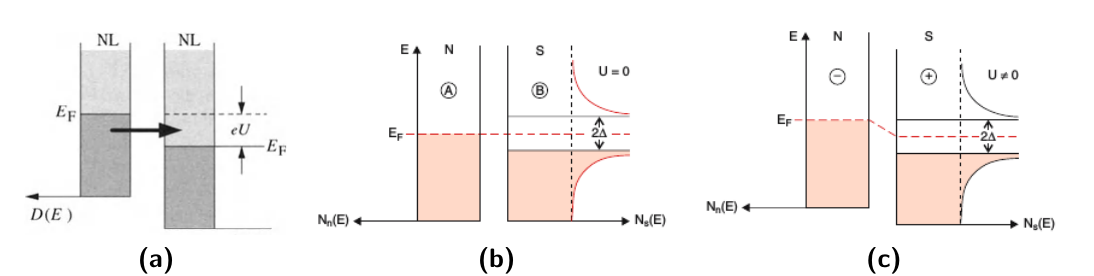
\includegraphics[scale=0.5]{tunnel.png}
\caption{d}
\label{fig:tunnel1}
\end{figure}

\begin{figure}[h]
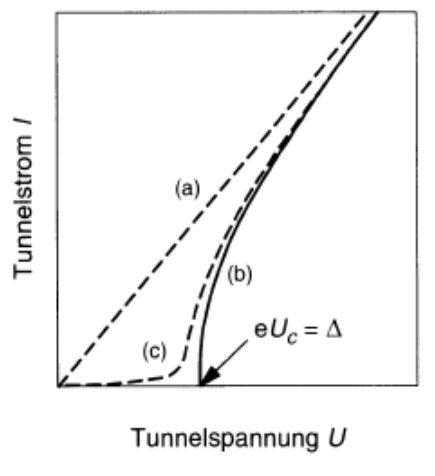
\includegraphics[scale=0.5]{kennlinie.png}
\caption{d}
\label{fig:tunnel2}
\end{figure}


\subsection{Vier Punkt Messung}

Dies ist eine Methode bei der die beiden Elektrodenpaar zur Strom und zur Spannungsmessung von einander getrennt sind.
\\
Damit eliminiert man den Leitungs sowie den Konataktwiderstand bei der Messung, was inbesondere bei der Messung kleiner Tunnelströme von Vorteil ist.


\subsection{Ablauf des Versuches}

\subsubsection{Herstellung der Probe}

Zunächst muss das Substat hergestellt werden, dass später bei der Messung verwendet wird.
Zu diesem Zweck wird eine Aufdampfanlage verwendet. 
Diese besteht im Wesentlichen aus einer Vakuumglocke in der sich verschiedene über externe Motoren bewegbare Komponenten befinden, wie etwa eine eine Halterung für das (Roh)($\equiv$ Si02) Substat.
\\
Nachdem man das Substat in der dafür vorgesehenen Halterung befestigt mit Ausdampfschablone hat, wird die Kammer mit zwei Vakuumpumpen für verschiene Druckbereiche evakuiert auf ungefähr $10^{-5} \text{ bar}$, was effizienter ist als nur eine Pumpe einzusetzen.
\\
Nun wird als erstes durch Bedinung der Anlange die eine Goldelektrode erhitzt eine circa $100 \text{ nm}$ dünne Schicht auf das Substat aufgedampft ($\equiv$ gesputtert).
Die Dicke kann hier
















\subsection{NL-NL Kennlinie}

Wie im Theorieteil angespochen erwarten wir bei Raumtemperatur das unspektakuläre ohm'sche Verhalten. 
Also einen linearen Zusammenhang zwischen Strom und Spannung.
Da es ohne Spannungsdifferenz keinen Strom gibt verläuft die Gerade zudem durch den Ursprung.
Durch lineare Regression ergibt sich zudem die Möglichkeit den Wiederstand oder die Leitfähigkeit des Tunnel-Kontaktes 2 zu berechnen.
\\
Die Steigung ergab einen Wert von $m = (0.00759  \pm 0.000003)  \frac{A}{V}$ für die Leitfähigkeit. Wobei wir für den Strom einen maximalen Fehler von $ \sigma_{I}=0.0001 A$ angenommen haben. 
Der y-Achsenachschnitt ist wie erwartet sehr klein, was auch aus der Abb. \ref{fig:NLNL} in der die Daten ebenso wie der lineare Fit geplottet sind, deutlich wird.
Aus der Steigung berechnet sich ein Widerstand von $R=(131.72 \pm 0.05) \Omega$ wobei $\sigma_{\Omega} = \frac{\sigma_{m}}{L} $.

\begin{figure}[h]
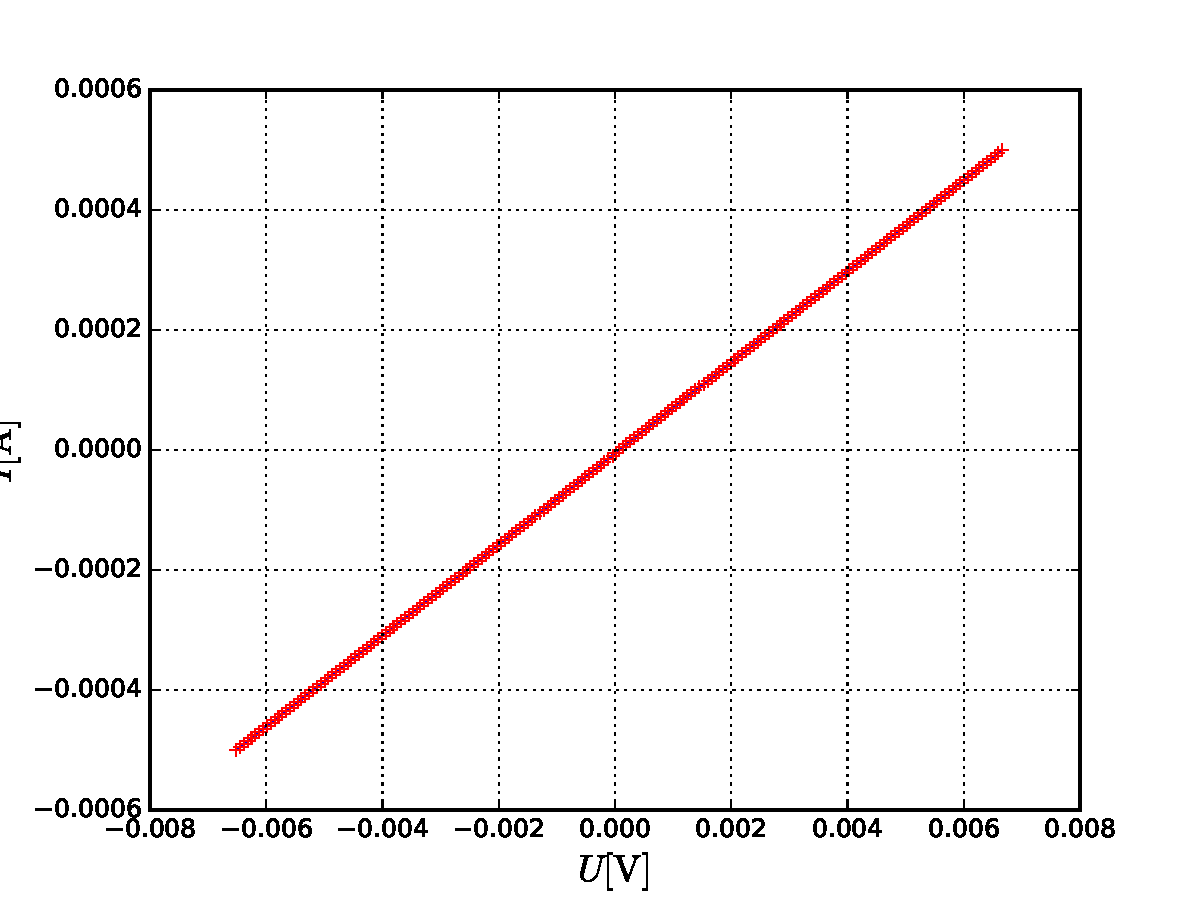
\includegraphics[scale=0.5]{1.pdf}
\caption{d}
\label{fig:NLNL}
\end{figure}

Wie sich die anderen Tunnelkontakte verhalten bei hohen Temperaturen können wir nicht beurteilen, da uns die entsprechenden Messdaten Fehlen.

\subsection{SL-NL Kennlinie}

Als nächstes wurde die U-I Kennlinie des gleichen Kontaktes bei niedrigen Temperaturen vermessen. Zudem ist zum Vergleich der oben diskutierte Verlauf bei Raumtemperatur ($\approx 25^{\circ} C$). In Abb. \ref{fig:SLNL} ist erkennbar, dass der erwähnte Hochtemperaturverlauf in etwa eine asymptotische Grenze für die Verläufe unterhalb der Sprungtemperatur darstellt.


\begin{figure}
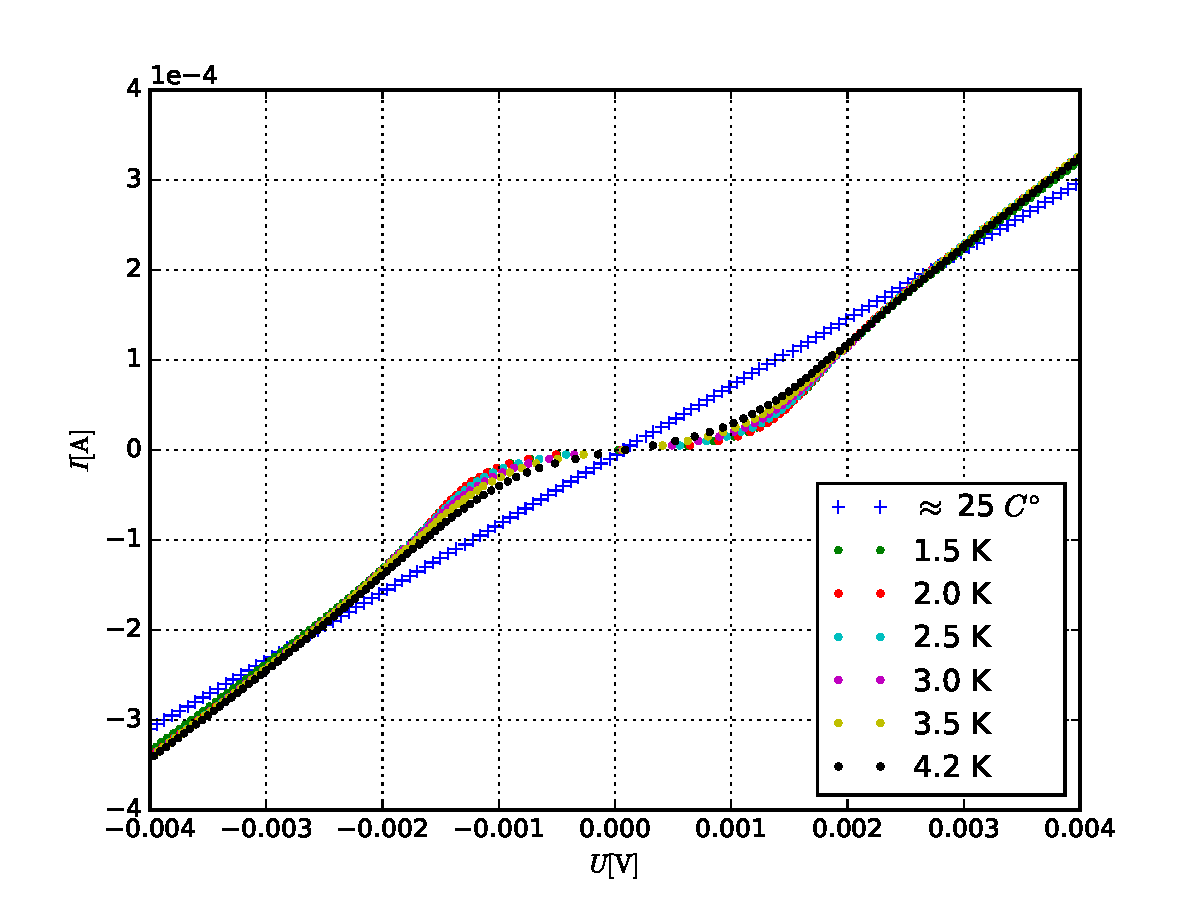
\includegraphics[scale=0.5]{2.pdf}
\caption{d}
\label{fig:SLNL}
\end{figure}
Die es wurden neben der Raumtemperatur sechs andere Temperaturen untersucht:
\\
$1.5 \text{ K}, 2.0 \text{ K}, 2.5 \text{ K}, 3.0  \text{ K}, 3.5 \text{ K}, 4.2 \text{ K}$
Es wird aus dem Verlauf des Graphen deutlich, dass zunächst eine gewisse Energiebarriere überwunden werden muss, bis ein Strom fließen kann, wenn eine Temperatur unterhalb von $T_C$ vorliegt.
Der Grund dafür ist, dass zunächst eine charakteristische Energie $2 \Delta$ für das aufbrechen der Cooperpaare aufgebracht werden muss, siehe Abb. \ref{fig:tunnel2}. 
Den nur so können die Elektronen, welche sich noch nicht im gepaarten Zustand vorliegen die Energielücke von $2 \Delta$(siehe Abb.) überwinden \ref{fig:tunnel1}. Dies ist der Grund weshalb beispielsweise in dem Intervall $0-0.001 V$ fast garkein Strom fließt. 
Zudem beobachtet man, dass der Verlauf in diesem Regime umso flacher ist je niedriger die Temperatur, siehe Abb. \ref{fig:SLNLB} für eine Detailansicht.
Dies entspricht auch den Erwartungen die wir aus der theoretischen Betrachtung gewonnen haben, denn bei $T > 0$ sind bereits manche Zustände oberhalb der Fermikante besetzt und der Verlauf wird etwas verschmiert.

\begin{figure}
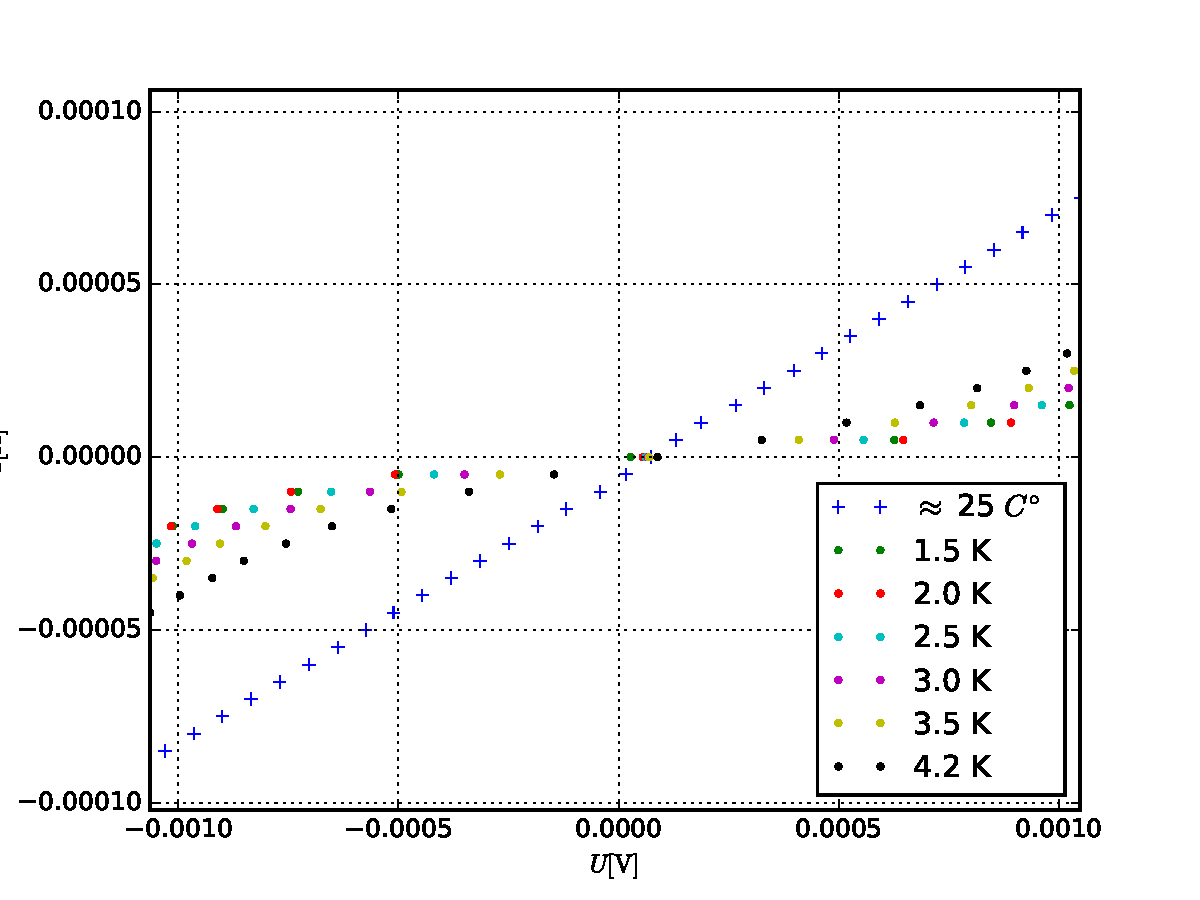
\includegraphics[scale=0.5]{2B.pdf}
\caption{d}
\label{fig:SLNLB}
\end{figure}

Für größere Ströme folgt der Verlauf des Stromes in etwa wieder wieder dem Ohmschen Gesetz.
\subsection{Bestimmung der Energielücke}

Um die Enegielücke zu bestimmen muss die Ableitung des gemessenen Verlaufes für den Strom nach der angelegten Spannung berechnet werden.
Zu diesem Zweck wurde numerische Ableitung mittels Python berechnet.
Das Skript verwendet den zentralen Differenzialquotienten
($\equiv$ MW aus rechtssiger und linksseitger Ableitung) in der diskretisierten Form:
\begin{align*}
\frac{d I}{d U} \approx \frac{1}{2} 
\left(
\frac{I_{j+1}-I_{j}}{U_{j+1}-U_{j}} 
+
\frac{I_{j}-I_{j-1}}{U_{j}-U_{j-1}}
\right)
\end{align*}

\begin{figure}
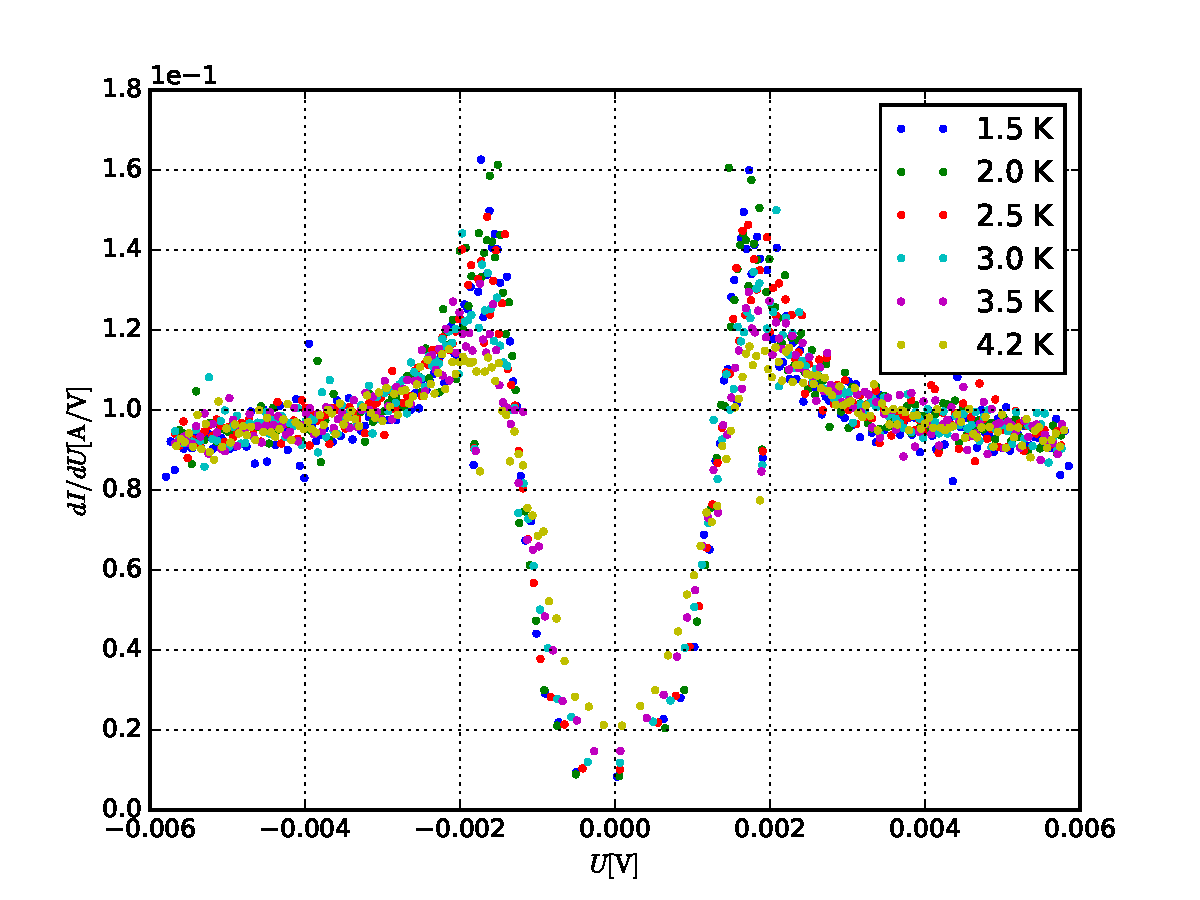
\includegraphics[scale=0.5]{3.pdf}
\caption{d}
\label{fig:SLNLDIF}
\end{figure}

Mit dieser Definition der Ableitung ergibt sich der Verlauf in Abb. \ref{fig:SLNLDIF}.
Nun können die Maxima dieses Verlaufes aus den Daten abgelesen werden
und die dazu gehörenden Werte für die Spannung, um den Spannungs
Bereich abschätzen zu können in dem für den supraleitenden Fall näherungsweise noch kein Strom fließt. Daher ergibt sich so für jede Messreihe einer 
Temperatur ein Wert für die Bandlücken energie durch
\begin{align}
\Delta \approx \frac{e(U_{rechts}-U_{links})}{2}
\end{align}
Da wir als einfache Schätzung die rechten und linken Maxima jedes Messreihe
als gute Werte angenommen haben wird der Fehler als relativ groß
angenommen und als Abstand zum nächstliegenden Spannungswert gesetzt.
Dies haben wir für alle Messungen als 0.01 mV eingeschätzt.

\begin{table}[]
\centering
\caption{My caption}
\label{my-label}
\begin{tabular}{|l|l|l|l|l|}
\hline
Temperatur K & $ 2 \Delta(T)$ V      & $\frac{2\Delta (T)}{k_{B} T_{C}}$ (fehler noch in mV)& $\Delta (T)_{k}$ V                              & $\frac{2\Delta (T)}{k_{B} T_{C}}$         \\ \hline
1.5  $\pm$ 0.075        & 0.00345875 $\pm$ 0.01 & 5.22459439 $\pm$ 0.16117          & 0.001552170836317999+/-1.5137903081638307e-05,  & 5.003389108154396+/-0.04879670306049267,  \\ \hline
2.0 $\pm$ 0.2         & 0.00298109 $\pm$ 0.01 & 6.01767483 $\pm$ 0.16117          & 0.0011918613212768532+/-2.2522078892686826e-05, & 3.8419391820639657+/-0.07259943402362494, \\ \hline
2.5     $\pm$ 0.125     & 0.00336755 $\pm$ 0.01 & 5.20444282 $\pm$ 0.16117          & 0.0013649042240310165+/-2.8330193099074682e-05, & 4.399739235141513+/-0.09132176450375008,  \\ \hline
3.0   $\pm$ 0.15       & 0.00405271 $\pm$ 0.01 & 3.92451077 $\pm$ 0.16117          & 0.0016579509847428388+/-3.296574312610501e-05,  & 5.344369127946088+/-0.10626435972127588,  \\ \hline
3.5   $\pm$ 0.175       & 0.00346762 $\pm$ 0.01 & 4.96357323 $\pm$ 0.16117          & 0.0011170828829334437+/-5.646896850335603e-05,  & 3.600892503967794+/-0.1820264982098407,   \\ \hline
4.2  $\pm$  0.21       & 0.00387855 $\pm$ 0.01 & 4.20121737 $\pm$ 0.16117          & 0.0008622164802902451+/-0.00010072756593996296  & 2.779336169328468+/-0.32469312946919865   \\ \hline
\end{tabular}
\end{table}



\subsection{BCS-Theory}

http://physics.stackexchange.com/questions/192416/interpolation-formula-for-bcs-superconducting-gap

Die BCS liefert den folgenden Zusammenhang für die Enegielücke $\Delta$, die Temperatur sowie der Besetzung $N(0)$ bei der Fermienergie:

\begin{align}
\frac{1}{N(0) V} = \int_{0}^{\hbar \omega_c} \frac{\tanh \left( \frac{1}{2} \beta (\epsilon^2 + \Delta^2)^(1/2) \right) }{(\epsilon^2 + \Delta^2)^(1/2)}
\label{eq:genauer}
\end{align}
Wenn man diese Formel nutzen möchte um daraus $\Delta(T)$ zu bestimmen, wie also die Gapenergie von der Temperatur abhängt, so würde man folgende Schritte berücksichtigen müssen:
\begin{itemize}
\item Numerische Integration 
\item Suchen einer Nullstelle, also $\frac{1}{N(0) V} - \text{Integral}(\Delta, T) = 0$
\end{itemize}
Dies müsste man über ein ganzes Intervall wiederholen, sodass man dann den Verlauf der Funktion $\Delta(T)$ berechnen kann.
\\
Es stellt sich aber heraus, dass es wesentlich einfacher ist folgende Näherungsformel für die Temperaturabhängigkeit der Energielücke zur verwenden
\footnote{Dies wird näher beschrieben in:
    Nature Materials
    10,
    849–852
    (2011)
    doi:10.1038/nmat3116}
:
\begin{align}
\Delta(T) = \Delta_{0} \tanh \left( k \sqrt{\frac{T_{c}-T}{T}} \right)
\end{align}
Die Abweichung von den numerisch besseren Werten, die man aus \ref{eq:genauer} erhält ist im untersuchten Temperaturbereich hinreichend klein. 
Damit reicht diese Formel für einen Vergleich der BCS Theorie vollkommen aus.
\\
Zudem sagt die BCS Theorie einen Wert für die Gap Energie bei $T=0$ voraus und gibt dies als Verhältnis zur kritischen Temperatur an:
\begin{align}
\Delta_{0}
=
\Delta(T=0)
= 1.76 k_{B} T_{C}
\end{align}
Mit $k \approx1.74$ als Parameter der sich für diese Näherungsformel ergibt.
Die Sprungtemperatur von Blei beträgt $T_{C} = 7.193 K$ 
\footnote{Charles Kittel: Introduction to Solid State Physics}.

\begin{figure}[h]
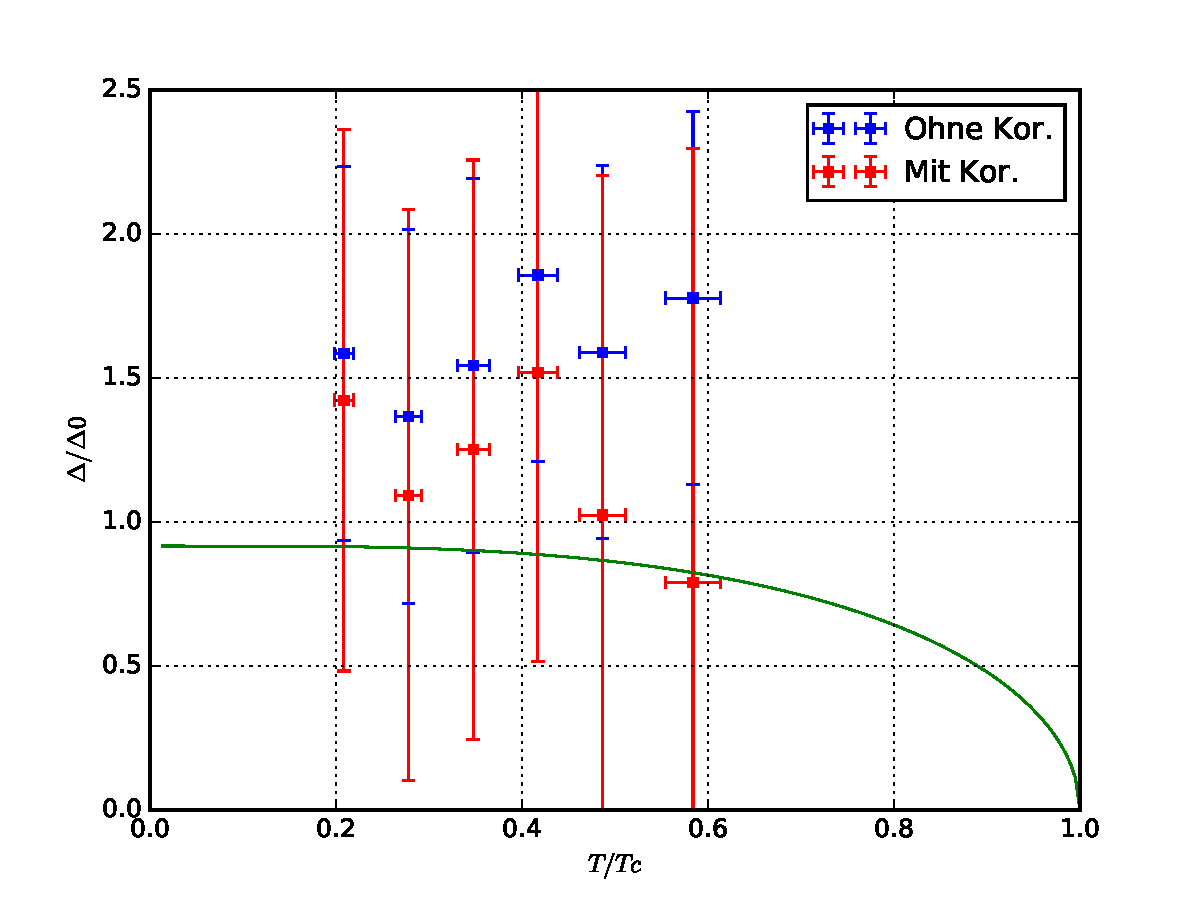
\includegraphics[scale=0.5]{4.pdf}
\caption{d}
\label{fig:NLNL}
\end{figure}

%\appendix
%
%\section{Anhang}
%
%
%\ldots
%
%\clearpage

% nicht unbedingt erforderlich
%\listoffigures
% nicht unbedingt erforderlich
%\listoftables

\bibliography{lit}

\end{document}